\newpage
\section{Progettazione}
\subsection{Studio dell'utenza finale}
\subsubsection{Utente generico}
L'utente generico che ci si può aspettare nel sito è di profilo informatico media alto ed è alla ricerca di informazioni riguardanti serie tv. L'utente generico registrato può commentare e lasciare un voto alla serie tv.

%\subsubsection{Azienda business-to-business}

\subsubsection{Amministratore}
Descrizione della pagina amministratore 

\subsection{Layout del sito}


\paragraph{Barra di navigazione}
~\\Il sito è stato pensato per avere una navigazione a barra orizzontale fissa posta in alto sullo schermo. Le pagine del sito sono, per quanto riguarda gli utenti non registrati:
\begin{itemize}
	\item \textbf{\normalsize{Esplora}}
	\item \textbf{\normalsize{Profilo}}
	\item \textbf{\normalsize{Preferiti}}
	\item \textbf{\normalsize{Impostazioni}}
	\item \textbf{\normalsize{FAQ}}
	\item \textbf{\normalsize{Supporto}}	
	\item \textbf{\normalsize{Privacy}}
	\item \textbf{\normalsize{About}}
\end{itemize}

Nella barra è presente il logo del sito e i pulsanti che portano alle altre pagine del sito. Nell'immagine sottostante è possibile vedere un esempio della barra di ricerca posta a sinistra della pagina: 
\begin{figure}[h!]  				% scheletro di ogni paragrafo
	\centerline{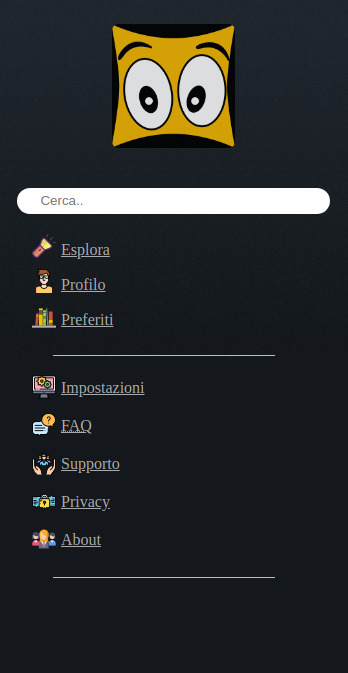
\includegraphics[scale=0.45]{img/nav_bar.png}}
	\caption{Barra di navigazione per utente generico}
	\label{fig:navbarGU}
\end{figure}
~\\

\newpage

\paragraph{Corpo}
~\\

\begin{figure}[h!]
	%\centerline{\includegraphics[scale=0.40]{img/corpo_esempio.jpg}}
	\caption{Esempio di sezione del corpo, aggiungere immagine sito}
	\label{fig:corpoGU}
\end{figure}
\paragraph{Pié di pagina}
~\\

\begin{figure}[h!]
	%\centerline{
\includegraphics[scale=0.45]{img/footer.png}}
	%\caption{Pié di pagina del sito}
	\label{fig:footer}
\end{figure}
\subsubsection{Amministratore}
Capire come va strutturata la pagina di amministratore 
\paragraph{Barra di navigazione}
~\\

\begin{figure}[h!]
	%\centerline{\includegraphics[scale=0.49]{img/barra_navigazione_admin.jpg}}
	\caption{Barra di navigazione per l'amministratore}
	\label{fig:navbarAD}
\end{figure}
\paragraph{Corpo}
\begin{figure}[h!]
	%\centerline{\includegraphics[scale=0.49]{img/add_form.jpg}}
	\caption{Form di aggiunta informazioni}
	\label{fig:addForm}
\end{figure}

\paragraph{Pié di pagina}
~\\
\subsection{Pagine per tipologia di utente}

\subsubsection{Utente generico}
\paragraph{Contenuti statici}

\subparagraph{About} 
~\\	
La pagina presenta le informazioni riguardanti la piattaforma e dei membri del gruppo. Sono poi presenti delle foto dei membri del gruppo con una breve descrizione riguardante il ruolo.
~\\	
\subparagraph{Supporto} 

~\\

\paragraph{Contenuti dinamici}   
\subparagraph{Esplora}

~\\
\subparagraph{Profilo}

~\\
\subparagraph{Preferiti}

~\\
\subparagraph{Impostazioni} 

~\\
\subparagraph{FAQ} 

~\\

\subparagraph{Privacy} 

~\\


%\subsubsection{Amministrazione}
%\paragraph{Pannello amministrazione} 
%\paragraph{Prodotti}
%~\\
%\paragraph{Servizi}
%~\\
%\paragraph{Amministratori}
%~\\
%\paragraph{Clienti}
%~\\

%\paragraph{Prenotazioni}
%~\\

%\paragraph{Storico prenotazioni}
%s~\\










